\documentclass[12pt]{article}
\usepackage{amsmath}
\usepackage{amssymb}
\usepackage{amsthm}
\usepackage{amsfonts}
\usepackage{graphicx}
\usepackage{textcomp}
\usepackage{hyperref}
\usepackage{tikz}
\usepackage{enumitem}
\usepackage{mathtools}
\usepackage{enumitem}
\usepackage{wasysym}
\usepackage{ulem}
\usepackage{xspace}
\usepackage{booktabs}
\usepackage{physics}

\ifPDFTeX % ensure generation of machine readable output
\input{glyphtounicode}
\pdfgentounicode=1
\usepackage[T1]{fontenc}
\usepackage[utf8]{inputenc}
\usepackage{lmodern}
\fi

\usepackage{csquotes}

\DeclareMathOperator{\dist}{dist}
\DeclareMathOperator{\Nul}{Nul}
\DeclareMathOperator{\Row}{Row}
\DeclareMathOperator{\proj}{proj}

\setlength{\arraycolsep}{12pt}

\newcommand{\defn}{\textbf{Def.}\xspace}
\newcommand{\thm}{\textbf{Thm.}\xspace}
\newcommand{\ex}{\textbf{ex.}\xspace}
\newcommand{\Ex}{\textbf{Ex.}\xspace}
\newcommand{\ie}{\textbf{i.e.}\xspace}
\newcommand{\lemma}{\textit{Lemma}\xspace}
\newcommand{\bproof}{\textit{Proof ($\impliedby$).}\xspace}
\newcommand{\fproof}{\textit{Proof ($\implies$).}\xspace}
\newcommand{\bigEps}{\mathcal{E}}
\newcommand{\soln}{\textit{Soln.}\xspace}

\renewcommand{\arraystretch}{1.25} % Adjust row spacing

\hypersetup{
    colorlinks=true,
    linkcolor=blue,
    filecolor=blue,      
    urlcolor=blue,
}

\newcommand{\ulhref}[2]{\href{#1}{\color{blue}\uline{#2}}}

\begin{document}

\title{MACM 316 Lecture 32}
\author{Alexander Ng}
\date{Monday, March 31, 2025}

\maketitle

\section{A continuation on the Elementary Theory of Initial Value Problems}

\subsection{Lipschitz Conditions}

\defn A function $f(t,y)$ satisfies a Lipschitz condition in the variable $y$ on
a set $D \in \mathbb{R}^2$ if a constant $L > 0$ exists such that

\[
  |f(t,y_1) - f(t, y_2)| \leq L|y_1 - y_2| \qquad \text{for all } (t,y_1), (t,y_2) \in D
.\]

The constant $L$ is called a \uline{Lipschitz Constant} for $f$.

*Examples can be found in the lecture notes for Lecture 31-b.*

\subsection{Convex Sets}

\defn A set $D\in \mathbb{R}^2$ is said to be \uline{convex} if whenever $(t_1,
y_1)$ and $(t_2,y_2)$ belong to $D$, the point
\begin{equation*}
  ((1-\lambda)t_1 + \lambda t_2, (1-\lambda)y_1 + \lambda y_2)
.\end{equation*}

\noindent
also belongs to $D$ for each $\lambda\in[0,1]$. Geometrically, a set is convex
if, for any two points in the set, a line segment connecting them lies entirely
within the set. (\ie every point in the set has line of sight to every other
point within the set.)

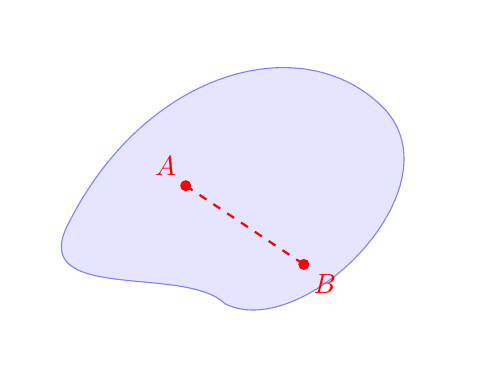
\begin{tikzpicture}

  % Draw the convex set as a smooth closed shape
  \filldraw[fill=blue!10, draw=blue!50] 
    (0,0) .. controls (1,2) and (3,2.5) .. (4,1.5)
    .. controls (5,0.5) and (3,-1.5) .. (2,-1)
    .. controls (1.5,-0.5) and (-0.5,-1) .. (0,0);

  % Two arbitrary points inside the convex set
  \fill[red] (1.5,0.5) circle (2pt) node[above left] {$A$};
  \fill[red] (3,-0.5) circle (2pt) node[below right] {$B$};

  % Line segment connecting the two points
  \draw[thick, red, dashed] (1.5,0.5) -- (3,-0.5);

\end{tikzpicture}

\subsubsection{Exercise 1 (22.5)}

Show that the set
\begin{equation*}
  D = \{(t,y):a\leq t\leq b, -\infty < y < \infty\}
.\end{equation*}
where $a$ and $b$ are constants, is convex.

To prove analytically, we can use the definition of convexity and show that each
point falls within the set.

\subsection{Theorem 1 (22.6)}

Suppose $f(t,y)$ is defined on a convex set $D\in \mathbb{R}^2$. If a constant
$L>0$ exists with
\begin{equation*}
  \abs{\frac{\partial f}{\partial y}(t,y)} \leq L
\end{equation*}

\noindent
then for all $(t,y) \in D$ then $f$ satisfies a Lipschitz condition on $D$ in
the variable $y$ with Lipschitz constant $L$.

\proof Let $(t, y_1)$ and $(t, y_2)$ be in $D$. Holding $t$ fixed, define 
$g(y) = f(t, y)$.

Suppose $y_1 \leq y_2$. Since the line joining $(t, y_1)$ to $(t, y_2)$ lies in
$D$ and $f$ is continuous on $D$ we have $g \in C[y_1, y_2]$. Furthermore,
\[
g'(y) = \frac{\partial f(t, y)}{\partial y}.
\]

Using the Mean Value Theorem on $g$, a number $\xi$ with $y_1 < \xi < y_2$ 
exists so that
\begin{align*}
  g(y_2) - g(y_1) &= g'(\xi)(y_2 - y_1) \\
  \implies f(t, y_2) - f(t, y_1) &= \frac{\partial f(t, y)}{\partial y}(y_2 - y_1) \\
  \implies \abs{f(t, y_2) - f(t, y_1)} &\leq L \abs{y_2 - y_1} \\
\end{align*}

So $f$ satisfies a Lipschitz condition on $D$ in the variable $y$ with Lipschitz
constant $L$. \qed

The previous theorem in combination with the next is particularly fundamental
for showing the existence and uniqueness of solutions to ODEs.

\subsection{Theorem 2 (22.7)}

Suppose that $D=\{(t,y): a\leq t \leq b, -\infty < y < \infty\}$ and that
$f(t,y)$ is continuous on $D$. 

If $f$ satisfies a Lipschitz condition on $D$ in the variable $y$, then the
initial value problem
\[
y'(t) = f(t, y(t)), \quad a \leq t \leq b, y(a) = \alpha
.\]
\noindent
has a unique solution $y(t)$ for $a \leq t \leq b$.

\subsubsection{Example (22.8)}
\noindent
\Ex Show that the IVP 
\[
y' = y\cos t, 0 \leq t \leq 1, y(0) = 1
.\]
\noindent has a unique solution.

\soln Since $f(t,y) = y\cos t$ we have $\frac{\partial f}{\partial y} = \cos t$.

$\implies f$ satisfies a Lipschitz condition in $y$ with $L=1$ on 
\[
D = \{(t,y): 0 \leq t \leq 1, -\infty < y < \infty\}.
.\]
Also, $f$ is continuous on $D$ --- $f$ is the product of continuous functions and
is therefore continuous --- so there exists a unique solution.

We also need to know if small changes in the statement of the problem introduce
correspondingly small changes in the solution.

\subsection{Theorem 3 (22.9)}

\thm The initial value problem
\begin{equation*}
  \frac{dy}{dt} = f(t,y), \quad a \leq t \leq b, y(a) = \alpha
.\end{equation*}
is said to be a well-posed problem if:

\begin{enumerate}
  \item A unique solution, $y(t)$, to the problem exists
  \item There exist constants $\bigEps_0 \geq 0$ and $k > 0$ such that for any $\bigEps$ with $\bigEps_0 > \bigEps > 0$, whenever $\delta(t)$ is continuous with
    \[
      |\delta(t)| < \bigEps \quad \text{for all } t \in [a, b]
    \]
    and when $|\delta_0| < \bigEps$, the initial value problem
    \[
      \frac{dz}{dt} = f(t, z) + \delta(t), \quad a \leq t \leq b, \quad z(a) = \alpha + \delta_0
    \]
    has a unique solution $z(t)$ that satisfies
    \[
      |z(t) - y(t)| < k\bigEps
    \]
    for all $t \in [a, b]$.
\end{enumerate}

The perturbed problem assumes the possibility of an error $\delta(t)$ being
introduced in the statement of the differential equation as well as an error
$\delta_0$ being present in the initial condition. Numerical methods also solve
perturbed problems since roundoff errors perturb the original problem.
$\implies$ It only makes sense to approximate well-posed problems.

\subsection{Theorem 4 (22.10)}
\thm Suppose $D=\{(t,y): a\leq t \leq b, -\infty < y < \infty\}$ 

If $f$ is continuous and satisfies a Lipschitz condition int he variable $y$ on
the set $D$, then the initial value problem
\[
\frac{dy}{dt}=f(t,y), \quad a \leq t \leq b, y(a) = \alpha
.\]
is well-posed.

\subsubsection{Example (22.11)}
\Ex Show that the initial-value problem
\[
y' = t^2y+1 , \quad 0 \leq t \leq 1, y(0) = 1
.\]
is well-posed.

\soln Since
\[
  \abs{\frac{\partial(t^2y+1)}{\partial y}} = \abs{t^2} \leq 1
.\]
and $t^2y+1$ is continuous --- it's a polynomial in $(t,y)$ --- we know that
this problem is well-posed.

\section{Euler's Method (23.1)}

Our first numerical scheme for intial value problems will be Euler's Method ---
a very simple but low order method.

Consider the initial value problem
% \[
% y' = f(t,y), \begin{cases}
%  y(a) = y_0 \\
%  a \leq t \leq b
% .\end{cases}
% .\]

\[
  \text{\textbf{IVP}}\begin{cases}
y' = f(t,y) & a \leq t \leq b\\
y(a) = y_0 & 
\end{cases}
\]

We will compute an approximation to the problem at the mesh points
\[
t_k = a + kh, \quad k = 0, 1, \ldots, N
.\]

where $h= \frac{(b-a)}{N}$ is called the \uline{step size}. Here we have assumed
$h$ is a constant, although variable step sizes are also useful

Euler's Method can be derived using a Taylor series expansion:
\begin{align*}
  y(t_{k+1}) &= y(t_k+h) = y(t_k) + hy'(t_k) + \frac{h^2}{2} y '' (\xi_k) \\
             &= y(t_k) + hf(t_k, y(t_k)) + \frac{h^2}{2}y''(\xi_k)
\end{align*}

Euler's Method constructs an approximation
\[
w_k \approx y(t_k)
.\]
by dropping the remainder term.
\begin{align*}
  w_0 &= y_0 \\
  w_k &= w_{k-1} + hf(t_{k-1}, w_{k-1}) \quad 1 \leq k \leq N\\
\end{align*}

\end{document}
